
The overall system schematic is shown in Figure \ref{fig0}. The only input to the system is the unstructured document or the raw text. An off-the-shelf Named Entity Recognizer (NER) first extracts the set of mentions from the raw text. These mentions are sent on to the Wikipedia API. In this paper, we use the Stanford NER \cite{stanford}, which was also the NER used by the authors of the state-of-the-art GLOW system \cite{roth}. The NER is available freely\footnote{\url{http://nlp.stanford.edu/software/CRF-NER.shtml}}. In the subsequent sections, we describe the remaining sub-modules that were used in the framework. 

\begin{figure}
\centering
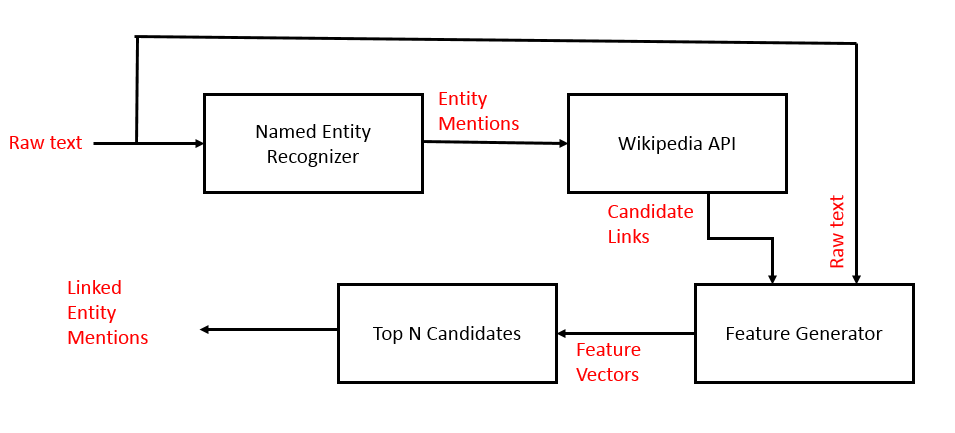
\includegraphics[height=5cm, width=12.5cm]{schematic}
\caption{The overall schematic of the proposed online wikifier.}
\label{fig0}
\end{figure}

\subsection{Wikipedia API}
Given a list of entity mentions that is output by the NER submodule, we rely on the 
Wikipedia API to extract (and return, via a REST protocol) the raw text of the candidate Wikipedia pages. Some 
named entities are ambiguous in the sense that they could refer to one of many different
Wikipedia articles. For example, the named entity `labour party' could refer to
`Social Democratic and Labour Party',
`Socialist Labor Party of America', or any number of other labour parties from many
different countries. For our particular application we are more focused on accuracy 
than coverage. Thus, when multiple candidates are returned,
we choose not to perform any linking. This conservative strategy leads to several links getting missed empirically, but the number is not as great as we might assume. Empirically, the majority of relevant mentions in the test suite (and in other documents we analyzed) had one candidate. We give specific statistics in Section \ref{experiments}. 

In its defense, the conservative decision was found to lead to fast wikification in practice, since less raw text has to be delivered over the Internet. Given that Wikipedia pages are quite long, adopting a liberal strategy\footnote{Getting all candidate links, with corresponding raw texts.} often led to payloads of a few megabytes getting returned \emph{per} page. Generating features and processing these pages (see the next section) was not instantaneous for such payloads, which is at odds with its online, real-time specification. The other usual assumptions for such payloads are, of course, sufficiently reliable REST calls to the API, as well as fast data connection. The conservative strategy minimizes the scope of these assumptions. 

Another motivation for the conservative strategy is that we empirically observed a significant slowdown when invoking the API too many times. Given that the system is intended for public deployment\footnote{The system is light enough that we are currently investigating a mobile app version for it, together with a browser extension. We believe that it is feasible to wikify and render annotated HTML pages as the user requests those pages, even on a cellular connection in a mobile browser.}, this is not a desirable trait. To improve recall, more sophisticated measures would have to be considered, but we leave for future work to determine the best way to achieve the performance improvement without burdening the online component. One such approach might be to set a threshold, such that mentions with more candidate links than the threshold number would get rejected. The conservative strategy is simply a special case of the former approach, with the threshold set to 1.  

Once obtained, the candidate pages, and also the original raw text, are input to the feature generator described in the next section. Our interface to the Wikipedia API is implemented in Python, and included with the other codebase and test suite on the companion page\footnote{\url{https://sites.google.com/a/utexas.edu/mayank-kejriwal/online-wikification}}.
\subsection{Feature Generator}
Features form the backbone of our system. A literature survey of existing wikifiers show that the primary difference between them lies in the complexity and expressivity of their features. Online wikification demands features that are simple yet representative. Towards this end, we devised three simple features to be used in conjunction with any n-gram model (including a bag of words model). The first of these is TF-IDF. The IDF is computed over the set of Wikipedia pages returned for the mentions in a raw text. Thus, a different IDF (an `on the fly' IDF) would be computed for each raw text document. We also experiment with TF and stop-words, that is, removing common stop-words before computing normalized TF vectors. Finally, we combined stop-words and IDF with TF. Note that the feature generator outputs a feature vector for each candidate Wikipedia page corresponding to a mention in the raw text and also outputs a feature vector for the raw text itself. The second (non-IDF) feature can be computed in a streaming fashion, but the other two require the first module to have finished retrieving all the candidates before calculating the feature vectors. We also assume that a small list of stop-words are provided to the system a priori. Such lists are quite extensively available\footnote{We used the one provided by \url{http://ir.dcs.gla.ac.uk/resources/linguistic_utils/stop_words} in our implementation.}. 
\subsection{Top N Candidates}
The goal of this module is to take the Wikipedia feature vectors and the raw text feature vector extracted by the feature generator  together with an additional user-provided input, N. Each Wikipedia feature vector is \emph{scored} by taking its dot product with the raw text feature vector. The top N Wikipedia vectors are marked as \emph{correct} and the corresponding mentions are linked to these Wikipedia pages. We experimentally show how accuracy varies with N in Section \ref{experiments}. 

Again, a threshold and weights can be specified instead of taking a simple dot product, but determining these would require training examples. Empirically, the hope is that by choosing a moderately small N, only the most important concepts in the page are wikified, and with high accuracy. We evaluate the success of these conservative design decisions in Section \ref{experiments}.


